% !TEX root = main.tex

% TODO:
% REMARK:

\section{ Systematic Uncertainty}
\label{sec:Systematic}

	Besides the statistical uncertainty, there are also some systematic uncertainty from detector's issue, reconstruction procedure, simulating process...etc. In this snalysis, the primary systematic uncertainties are from the simulation correction. 

	\subsection{Introduction of systematic uncertainty}
	\label{ssec:Syst_type}
		\subsubsection{Pileup re-weighting}
		\label{sssec:Syst_PU}

			% https://twiki.cern.ch/twiki/bin/viewauth/CMS/PileupMCReweightingUtilities?fbclid=IwAR0SuZFQ5Um0IfZn1-CHXia6NPMYe2_7cz2OGXxhCYvNvfl_tTBke-w22l8

			Since the pileup performance under data and simulation(MC) have discrepancy, there is MC reweighing of pileup in any events which is mentioned in section.\ref{sssec:DataAndMC_PU}. However, there is also an uncertainty of pileup reweight. The pp inelastic scattering cross section is used to calculate the pileup distribution and then used to implement the pileup reweight, so this cross section has its mean value and uncertainty 69.2$mb^{-1}$ $\pm$5\%. Then the pileup reweighing factor may be affected by this cross section as the pileup reweighting systematic uncertainty.

		\subsubsection{Jet energy correction and resolution}
		\label{sssec:Syst_JECJER}

			

		\subsubsection{b-tagged scale factor}
		\label{sssec:Syst_btag}

		\subsubsection{Lepton identification, isolation, reconstruction and trigger efficiencies}
		\label{sssec:Syst_JECJER}

			eee
	\subsection{Implementation and results}
	\label{ssec:Syst_imp_result}

		The approaches to apply the systematic uncertainty are shown below. First, we 

		\begin{figure}[H]
		\centering{}
	    	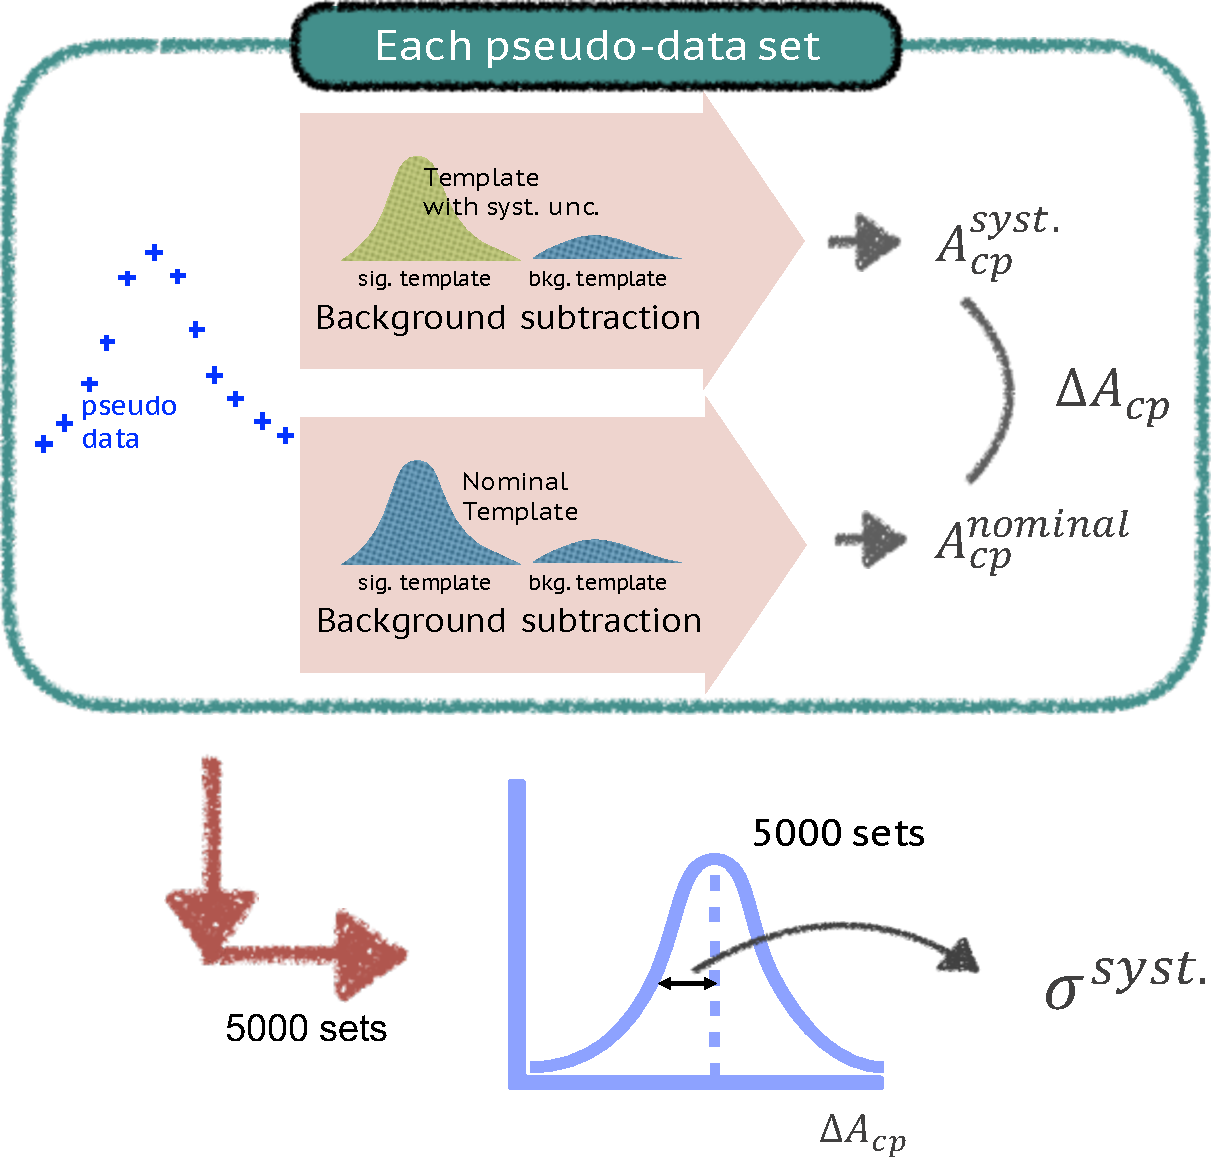
\includegraphics[width=0.85\textwidth]{Figures/SystUnc/approach_syst.pdf}\\
		\caption{Process of measuring systematic uncertainty}
		\label{BkgEst:fig:Bkt_sub}
		\end{figure}
		\FloatBarrier


\FloatBarrier
